\documentclass[a4paper,14pt]{extreport}

\usepackage[T1,T2A]{fontenc}
\usepackage[utf8]{inputenc}

\usepackage{title}
\usepackage{bsumain}
\usepackage{blindtext}

\usepackage{hyperref}
\usepackage{subfigure}
\usepackage[final]{graphicx}

\title{о прохождении производственной (преддипломной) практики}
\author{Бинцаровского Леонида Петровича}
\mentor{старший преподаватель\\
        Д. И. Пирштук}

\renewcommand\contentsname{Оглавление}

\begin{document}
    \maketitle\newpage
    
    \tableofcontents\newpage
    \chapter*{Введение}
    \addcontentsline{toc}{chapter}{Введение}
    Современные технологии стремительно развиваются, проникая во все сферы нашей жизни. Одной из ключевых задач становится обработка и анализ видеопотоков, что позволяет улучшать пользовательский опыт, создавать новые форматы взаимодействия и автоматизировать сложные процессы.
    
    В настоящее время обработка видеопотоков и редактирование контента стали неотъемлемой частью современной технологической среды. Одним из направлений в этой области является улучшение качества видеопотока. Есть множество вариантов: увеличение разрешения, стилизация в определённом стиле, удаление шума (denoising), улучшение цветопередачи, добавление эффекта глубины, автоматическое центрирование объекта и многое другое.

    На данный момент в большинстве сфер ит-направления применяются нейронные сети. И обработка видеопотока не осталась в стороне. Почти все вышеперечисленные варианты для улучшения качества видео могут быть реализованы с помощью нейронных сетей.

    Целью данной работы является описание и разработка архитектуры пайплайна для инференса выбранной модели на мобильных устройствах. Пайплайн должен обеспечивать высокую эффективность, как по скорости инференса и постобработки, так и по энергопотреблению.

    \chapter{Обзор существующих реализаций и основных нюансов для GPU пайплайна}
        Инференс нейронных сетей непосредственно на устройстве дает множество преимуществ, включая низкую задержку, устранение зависимости от сервера, низкие коммуникационные расходы и низкую стоимость системы. Благодаря этому инженеры могут реализовать на мобильных устройствах различные приложения, работающие в режиме реального времени, и чаще всего это работа с видеопотоками.
    
        Однако энергоэффективность является одной из основных проблем, с которой сталкиваются при таком подходе. Обычно нейросетевые модели требуют больших вычислительных затрат. Мобильные устройства имеют очень ограниченную ёмкость аккумулятора и возможности питания. Повышенное энергопотребление приводит к сокращению срока службы батареи или даже к тепловому дросселированию (один из компонентов системы, чаще всего процессор или видеокарта, достигает максимальной безопасной рабочей температуры).

        На смартфонах и ноутбуках большинство приложений подразумевают работу с графикой и изображениями, а связанная с ними обработка и визуализация данных в значительной степени зависят от графических процессоров. Чтобы улучшить возможности графического пайплайна и максимально эффективно использовать вычислительные ресурсы, распространённой стратегией является интеграция нейросетевых моделей в графические приложения. Однако существующие фреймворки для инференса не ориентированы на постобработку на мобильных устройствах. Входные и выходные данные также не являются текстурами GPU. Из-за этого накладные расходы на ввод/вывод, связанные с передачей данных между текстурами GPU и буферами ввода/вывода, невозможно избежать, что приводит к снижению производительности приложений в реальном времени и влияет на энергоэффективность.

        На текущий момент есть три основных фреймворка для инференса нейронных сетей на мобильных устройствах, таких как TensorFlow Lite (TF-Lite) \hyperlink{[1]}{[1]}, PyTorch Mobile \hyperlink{[2]}{[2]} и CoreML \hyperlink{[3]}{[3]}. Также в последние годы было предложено большое количество более облегчённых фреймворков. В 2020 году компания Alibaba разработала Mobile Neural Network (MNN) \hyperlink{[4]}{[4]}, которая является универсальной и оптимизирована для мобильных приложений. Другие разработки, такие как Tencent NCNN \hyperlink{[5]}{[5]}, Tencent TNN \hyperlink{[6]}{[6]}, Huawei Bolt \hyperlink{[7]}{[7]}, Xiaomi MACE \hyperlink{[8]}{[8]} и Baidu Anakin \hyperlink{[9]}{[9]}, также являются легковесными и не имеют большого количества сторонних зависимостей, что делает их довольно хорошей альтернативой для инференса на мобильных устройствах.

        Поскольку речь идет про обработку видеопотока на GPU, будут рассмотрены только соответствующие бэкенды. На iOS единственным GPU-бэкендом для инференса является Metal, который объединяет функции, схожие с OpenGL и OpenCL, в единый API. Для большинства телефонов на базе Android и ноутбуков вариантами работы на GPU являются OpenGL, Vulkan и OpenCL. OpenGL широко поддерживается почти всеми системами, оснащёнными GPU любого производителя. Vulkan — это кроссплатформенный API с низкими накладными расходами для 3D-графики и вычислений. Из-за того, что Vulkan является более низкоуровневым, он требует больших усилий от разработчиков для интеграции. OpenCL поддерживается на некоторых последних мобильных GPU, но пока не получил широкой поддержки. Среди этих GPU-бэкендов OpenGL наиболее широко распространён в мобильных устройствах.

        \begin{figure}[!h]
            \begin{center}
                \begin{minipage}[!h]{0.75\linewidth}
                    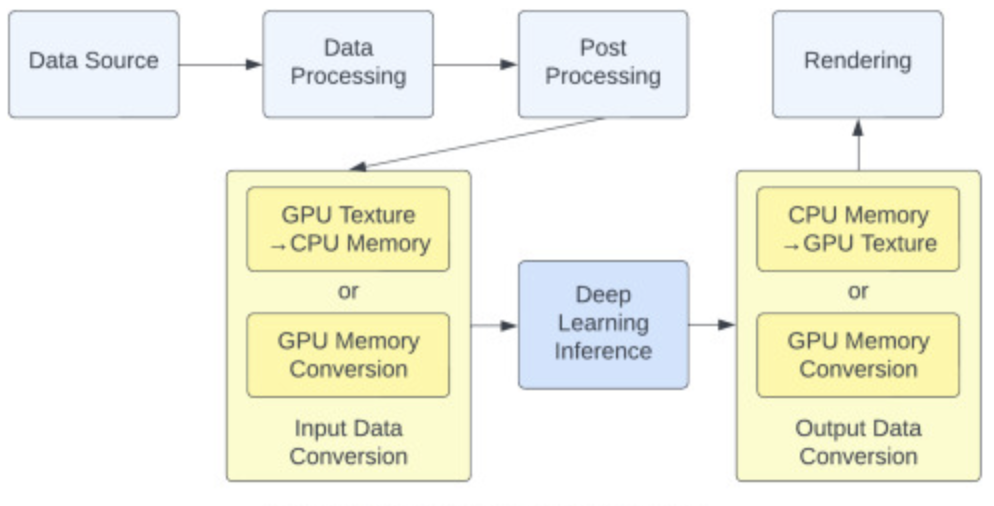
\includegraphics[width=1\linewidth]{images-pipeline/data.png}
                    \label{ris:netron}
                    \caption{Пайплайн реализованный на сторонних фреймворках \hyperlink{[13]}{[13]}}
                \end{minipage}
            \end{center}
        \end{figure}
        
        Несмотря на то, что почти во всех современных фреймворках существуют  несколько вариантов инференса на мобильных GPU, при интеграции их в реальный пайплайн возникают некоторые проблемы. Первая из них - это производительность. Из-за оптимизации кода одна и та же модель может иметь разные задержки на различных движках. Другая проблема связана с совместимостью. Некоторые модели могут не работать с GPU-бэкендом или работать медленно из-за отката к режиму CPU. Последняя, но не менее важная проблема - обмен данными. Все вышеперечисленные фреймворки для инференса принимают на вход Tensor или Mat, но эти структуры данных не могут напрямую работать с текстурами OpenGL. Это существенное ограничение, поскольку текстуры OpenGL широко используются в графике и приложениях для обработки изображений.
        
        Исходя из этого, будем рассматривать OpenGL как основной движок для описываемого конвейера.

        \section{Выбор и описание модели для построения конвейера}
        \begin{figure}[!h]
            \begin{center}
                \begin{minipage}[!h]{\linewidth}
                    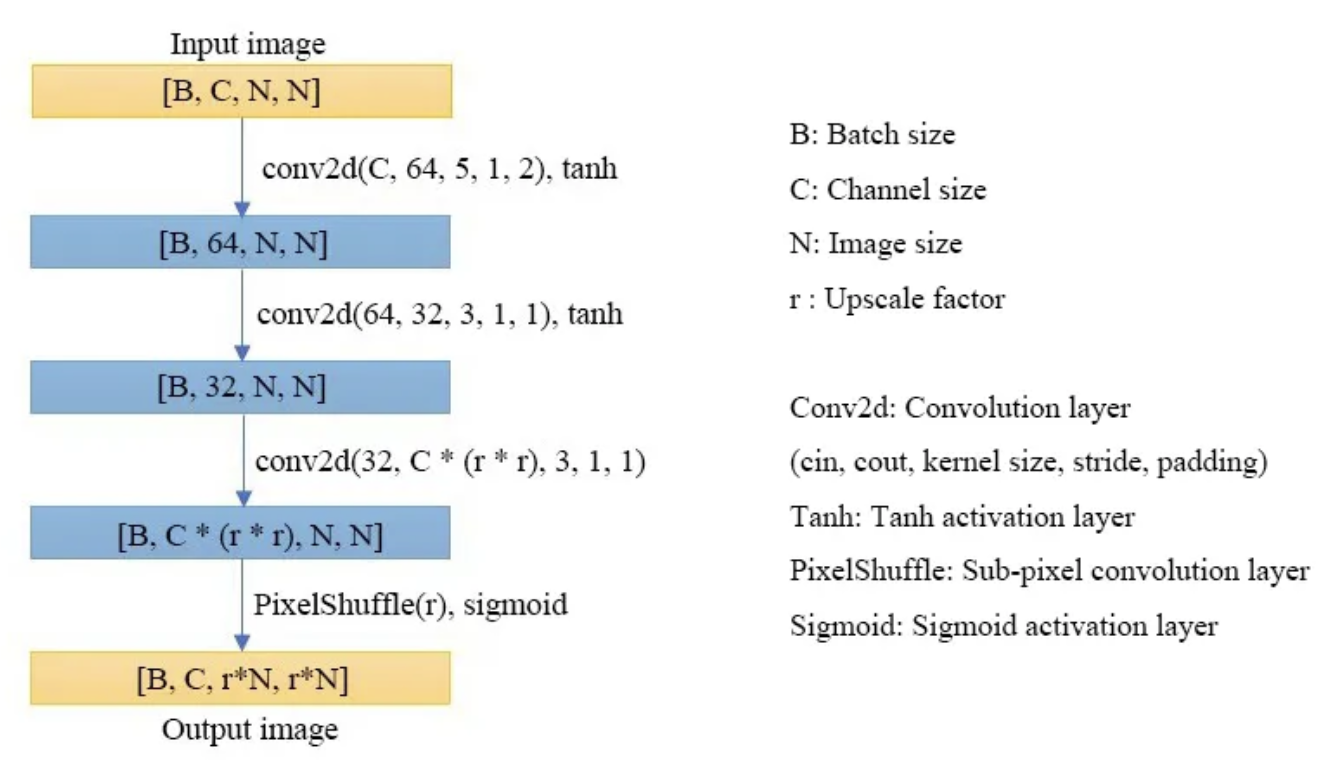
\includegraphics[width=1\linewidth]{images-pipeline/model.png}
                    \label{ris:netron}
                    \caption{Структура модели ESPCN \hyperlink{[10]}{[10]}}
                \end{minipage}
            \end{center}
        \end{figure}
        
        Для реализации рассматриваемого пайплайна была выбрана модель ESPCN \hyperlink{[10]}{[10]}. Архитектура сети ESPCN представляет собой L слоев, где первые L-1 слоя — это конволюционные слои, которые получают карты признаков входных изображений в низком разрешении, а  последний слой — эффективный subpixel convolutional слой для восстановления размера выходного изображения с заданным коэффициентом масштабирования.
        Обычно сеть состоит из 3 слоев:
        \begin{enumerate}
            \item Входное изображение с формой [B, C, N, N].
            \item Первый слой: конволюционный слой с 64 фильтрами и размером ядра $5 \times 5$, затем слой активации tanh.
            \item Второй слой: конволюционный слой с 32 фильтрами и размером ядра $3 \times 3$, за которым следует слой активации tanh.
            \item Третий слой: конволюционный слой с фиксированным числом выходных каналов $C \times r \times r$ и размером ядра $3 \times 3$.
            \item Применение функции перестановки subpixel'ей, чтобы выходное изображение имело вид [B, C, $r \times N$, $r \times N$], а затем слой активации sigmoid.
        \end{enumerate}

        \begin{figure}[!h]
            \begin{center}
                \begin{minipage}[!h]{0.39\linewidth}
                    \begin{center}
                        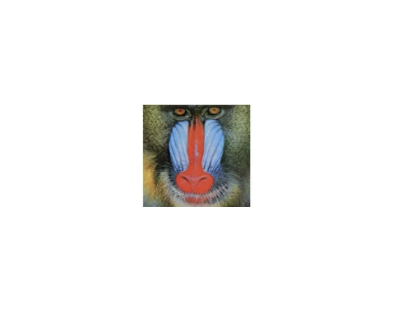
\includegraphics[width=1\linewidth]{images-pipeline/LR.png}
                        \label{ris:json}
                        \caption{Изображение в низком разрешении, передаваемое на вход модели \hyperlink{[10]}{[10]}}
                    \end{center}
                \end{minipage}
                \hfill
                \begin{minipage}[!h]{0.39\linewidth}
                    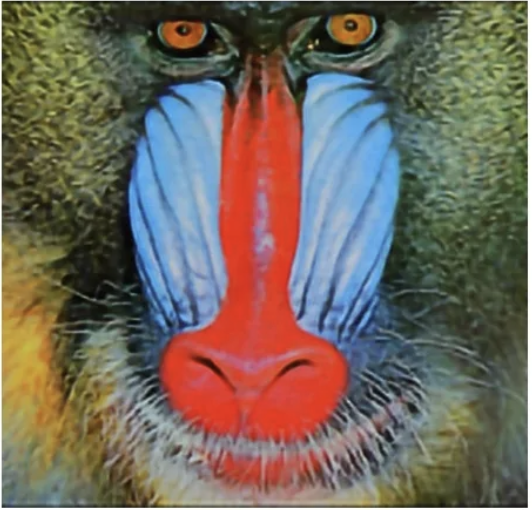
\includegraphics[width=1\linewidth]{images-pipeline/SR.png}
                    \label{ris:netron}
                    \caption{Результат обработки моделью ESPCN \hyperlink{[10]}{[10]}}
                \end{minipage}
            \end{center}
        \end{figure}
        
    \chapter{Архитектуры пайплайна}
        Разрабатываемый пайплайн можно разделить на четыре основных этапа:
        \begin{enumerate}
            \item Преобразование модели в удобный для работы формат;
            \item Загрузка модели и манипуляции с ней;
            \item Генерация вычислительного графа и необходимая предобработка;
            \item Выполнение соответствующих операторов для обработки модели.
        \end{enumerate}
        
        \section{Преобразование модели}
            \begin{figure}[!h]
                \begin{center}
                    \begin{minipage}[!h]{0.38\linewidth}
                        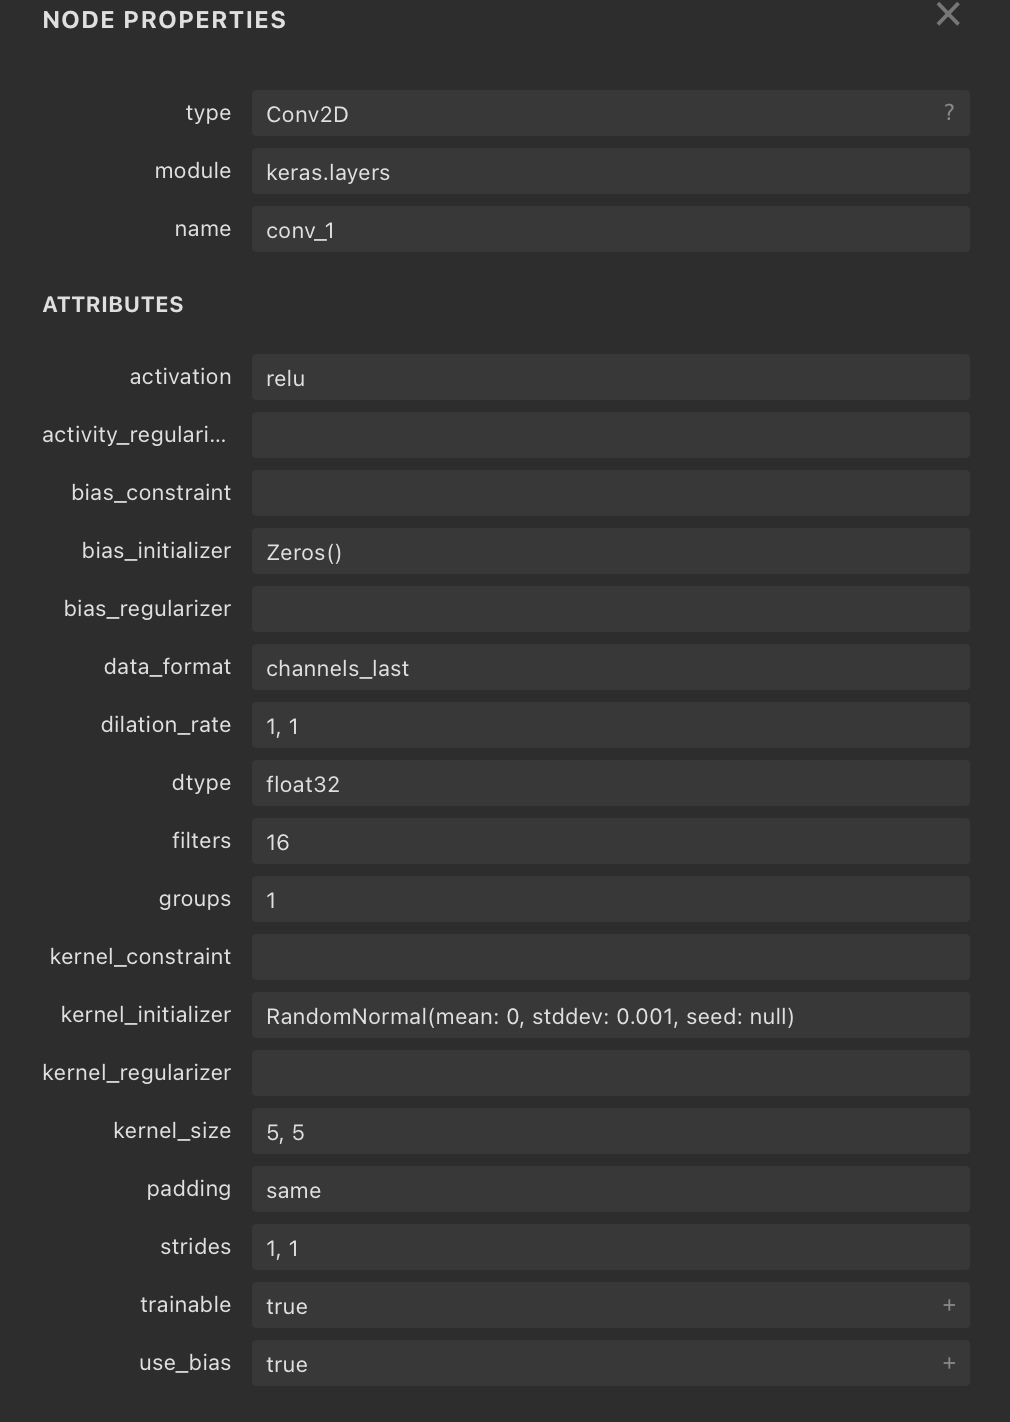
\includegraphics[width=1\linewidth]{images-pipeline/netron.png}
                        \label{ris:json}
                        \caption{Вид модели в веб-приложении Netron \hyperlink{[11]}{[11]}}
                    \end{minipage}
                    \hfill
                    \begin{minipage}[!h]{0.39\linewidth}
                        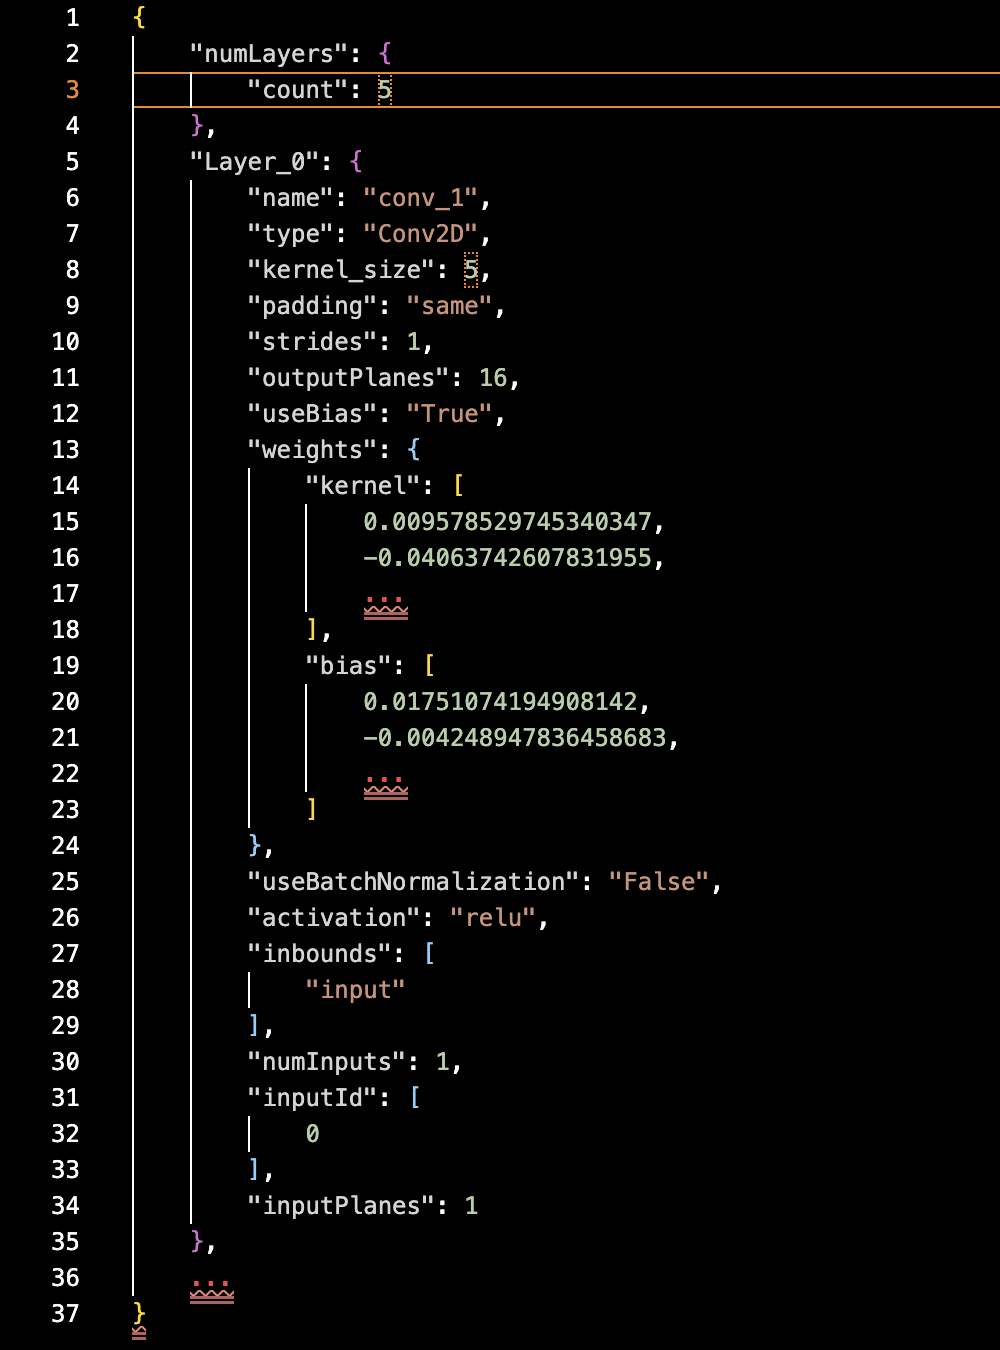
\includegraphics[width=1\linewidth]{images-pipeline/json.png}
                        \label{ris:netron}
                        \caption{Структура модели в созданном json файле} 
                    \end{minipage}
                \end{center}
            \end{figure}
            
            Так как большинство моделей обучается с помощью общедоступных фреймворков TensorFlow, Keras или PyTorch, они хранятся в соответствующих форматах. Следовательно, для их загрузки необходимо использовать один из перечисленных фреймворков, что является не совсем логичным в рамках разрабатываемого пайплайна из-за их размера. Поэтому для максимальной оптимизации и облегчения было принято решение о конвертации моделей в более удобный формат для загрузки — json файл. Для этого из модели необходимо извлечь всю необходимую информацию: количество слоев, тип слоя, входные параметры (ширина, высота, размер ядра), тип паддинга, веса текущего слоя, bias текущего слоя (дополнительная информация о природе данных для модели), какой тип активации использовать и т.д.

            Для этих целей был написан скрипт на языке Python, который на вход принимает модель в формате .h5 и возвращает json файл. Для его реализации используются сторонние библиотеки TensorFlow, для чтения входной модели, и json, для корректной работы со структурой файла и дальнейшей записи в соответствующий формат. Модель конвертируется один раз и далее пайплайн будет принимать только подготовленный формат (json файл). Также такой подход позволяет немного выиграть в памяти, требуемой для пайплайна. Во-первых, нет необходимости иметь стороннюю зависимость от TensorFlow, что отразилось бы на размере пайплайна. Во-вторых, json файл можно загрузить в память статически, что позволит избавиться от внешних зависимостей.
            
        \section{Загрузка модели и манипуляции с ней}
            Для загрузки модели были реализованы вспомогательные классы. Их основные функции заключаются в извлечении данных из json файла и хранении их в определенном формате в памяти. Класс ModelParser непосредственно отвечает за загрузку данных из файла и использует для этих целей доступный в открытом доступе фреймворк nlohmann::json. 

            При считывании графа из json файла применяется слияние слоев (эффективная оптимизация вычислительного графа). Данная техника позволяет значительно сократить количество слоев и, таким образом, снизить вычислительную стоимость инференса. Теоретически, если один из слоев представляет собой операцию element-wise или функцию map, он может быть объединен с предыдущим слоем. Например, слой activation можно объединить в один со слоем свертки или batch-нормализации, которые обычно за ним следуют.
            
            Также к такому методу можно прибегнуть и со слоем padding. Если его режим постоянный, повторяющийся или симметричный, то его можно объединить со следующим за ним. В следующем же слое объект OpenGL Sampler, прикреплённый к входной текстуре, обеспечит padding-функцию и тем самым уменьшит накладные расходы на проверку границ.

        \section{Архитектуры пиксельного шейдера}
            В графическом пайплайне OpenGL пиксельный шейдер — это этап, который обрабатывает отдельные фрагменты для определения значения цвета соответствующих пикселей, присутствующих в данном фрагменте. Выходом пиксельного шейдера являются значения глубины и цвета, которые обычно записываются в render target или в framebuffer. Этап пиксельного шейдера работает совместно с этапом вершинного, который отвечает за предоставление координат интересующей квадратной области для последующей обработки её уже пиксельным шейдером.

            В отличие от вычислительных шейдеров, которые являются более гибкими и могут использоваться для более широкого круга задач, пиксельные оптимизированы для рендеринга графики на экране (минус вычислительных шейдеров в том, что они менее универсальны, так как появились лишь в стандарте 4.6, который поддерживается не на всех устройствах). Этот тип рендеринга обычно предполагает параллельную обработку большого количества пикселей. По сравнению с вычислительными шейдерами, пиксельные продемонстрировали превосходство в производительности благодаря лучшей локальности данных и более эффективным схемам доступа к памяти. Например, в контекстно-зависимых алгоритмах, где каждое значение пикселя вычисляется и зависит от соседних значений, фрагментные (пиксельные) работают с областью в пространстве экрана, что позволяет им использовать преимущества локальности данных и потенциально повысить производительность.
            
            Кроме того, пиксельные шейдеры обращаются к текстурным данным, которые хранятся в специальном типе памяти, называемом текстурным кэшем. Чаще всего это быстрее, чем обращение к данным, хранящимся в глобальной памяти, особенно если обращение к текстурным данным происходит неоднократно.
            
            В сверточных нейронных сетях (CNN) наиболее часто встречающейся операцией и, в свою очередь, одной из самых сложных, является свертка. Свертка в двух измерениях или на изображениях — это контекстно-зависимый алгоритм, в котором выходное значение вычисляется как сумма произведений ядра и сэмплированных входных пикселей. Это делает фрагментный шейдер подходящим вариантом использования при разработке механизма вывода для развертывания CNN.

            Исходя из вышеперечисленных плюсов пиксельного шейдера и особенностей архитектуры ESPCN (она является разновидностью архитектуры CNN), было принято решение в реализуемом пайплайне использовать именно их.

            При переводе операций, выполняемых CNN, в реализуемый пайплайн, входные данные слоя будут находиться в текстуре и обрабатываются вершинным и пиксельным шейдером. Затем данные записываются в render target. В зависимости от количества каналов на входе и выходе, данные могут храниться либо как текстура 2D, хранящая 4 канала, либо как массив текстур 2D, хранящий ещё 4 канала. Для операции свертки в пиксельный шейдер веса будут передаваться через uniform buffer object или как входные uniform.
            
            Для универсальности, необходимые .glsl-файлы создаются непосредственно после извлечения данных из файла модели, при этом используются шаблоны (для каждого слоя они уникальны), написанные заранее. Для выбранной модели необходимо 3 шаблона: для слоя convolutional, activation и subpixel convolutional. Ниже приведен шаблон пиксельного шейдера для слоя activation:

            \lstinputlisting[language=c++, caption={Шаблон пиксельного шейдера для слоя activation}]{codePipeline/activation.glsl}

            В данном шаблоне присутствуют дефайны, которые определяют алгоритм работы шейдера. Например, в данном шейдере PLANE\_COUNT отвечает за количество выходных плоскостей для слоя активации. Данные для необходимых дефайнов будут заданы во время обработки модели из файла. Необходимо отметить и \_PLACEHOLDER\_UNIFORMS\_DECLARATION\_. Данная строка отвечает за местоположение входных uniforms. Во время сборки шейдера будет передан необходимый список uniform с соответствующими им входными параметрами. Данный подход сильно облегчает создание пиксельных шейдеров и делает этот процесс более универсальным.
            
            Также стоит отметить, что каждый шейдер отвечает за генерацию 4-канального вывода в render pass. Для расчета слоя, имеющего более 4 выходов, требуется несколько .glsl-файлов и render pass, что и пришлось реализовывать для выбранной модели. Ниже приведена таблица, в которой перечислены слои и соответствующие им количества render pass:

            \begin{table}[H]
                \begin{center}
                    \begin{tabular}{|l|l|}
                        \hline
                        Модель ESPCN & Количество render pass \\
                        \hline
                        Layer 1: Conv2D output: $n \times n \times 16$ & Layer 1 output: 4 render passes \\
                        \hline
                        Layer 2: Conv2D output: $n \times n \times 16$ & Layer 2 output: 4 render passes \\
                        \hline
                        Layer 3: Conv2D output: $n \times n \times 4$ & Layer 3 output: 1 render pass \\
                        \hline
                        Layer 4: Subpixel output: $2n \times 2n \times 1$ & Layer 4 output: 1 render pass \\
                        \hline
                    \end{tabular}
                \end{center}
                \caption{\label{tab:canonsummary}Соотношение слоев модели ESPCN и количество render pass}
            \end{table}

        \section{Архитектуры вершинного шейдера}
            Для корректной работы пиксельного шейдера необходимо создать соответствующий ему вершинный шейдер. В реализуемом пайплайне для всех слоев необходимо реализовать один общий вершинный шейдер. Он должен выделять необходимую квадратную область для рендеринга. Получаем такой вид:

            \lstinputlisting[language=c++, caption={Шаблон пиксельного шейдера для слоя activation}]{codePipeline/vertex.glsl}

            В данном коде можно заметить матрицу v, которая состоит из трех вершин формата vec4(x, y, z, w). При этом стоит отметить, что
            \begin{enumerate}
                \item x, y → позиция вершины на экране (в пространстве NDC);
                \item z, w → UV-координаты, передаваемые далее в v\_uv.
            \end{enumerate}

            Данные координаты точек выбраны не случайно, так как при них OpenGL автоматически отрежет лишнее и в результате полученный треугольник покроет весь экран. Этот способ позволяет покрыть весь экран без отрисовки двух треугольников, как в стандартной реализации. Ниже приведено пояснение каждой координаты:
            \begin{enumerate}
                \item (-1, -1) нижний левый угол — с uv (1, 1);
                \item (3, -1) далеко за правый нижний край — uv (1, -1);
                \item (-1, 3) далеко за верхний левый край — uv (-1, 1).
            \end{enumerate}
            
    \chapter*{Заключение}
    \addcontentsline{toc}{chapter}{Заключение}
    В ходе работы:
    \begin{enumerate}
        \item Был успешно произведен обзор существующих реализаций и основных нюансов для GPU пайплайна. Основные нюансы заключаются в отсутствии фреймворков с поддержкой аппаратных структур данных GPU для входа: нельзя без потерь по времени передать выход модели напрямую в рендер пайплайн. Данная операция происходит через конвертацию GPU->CPU->GPU, что довольно накладно. Поэтому принято решение использовать GPU only пайплайн с использованием движка OpenGL;
        \begin{figure}[!h]
            \begin{center}
                \begin{minipage}[!h]{\linewidth}
                    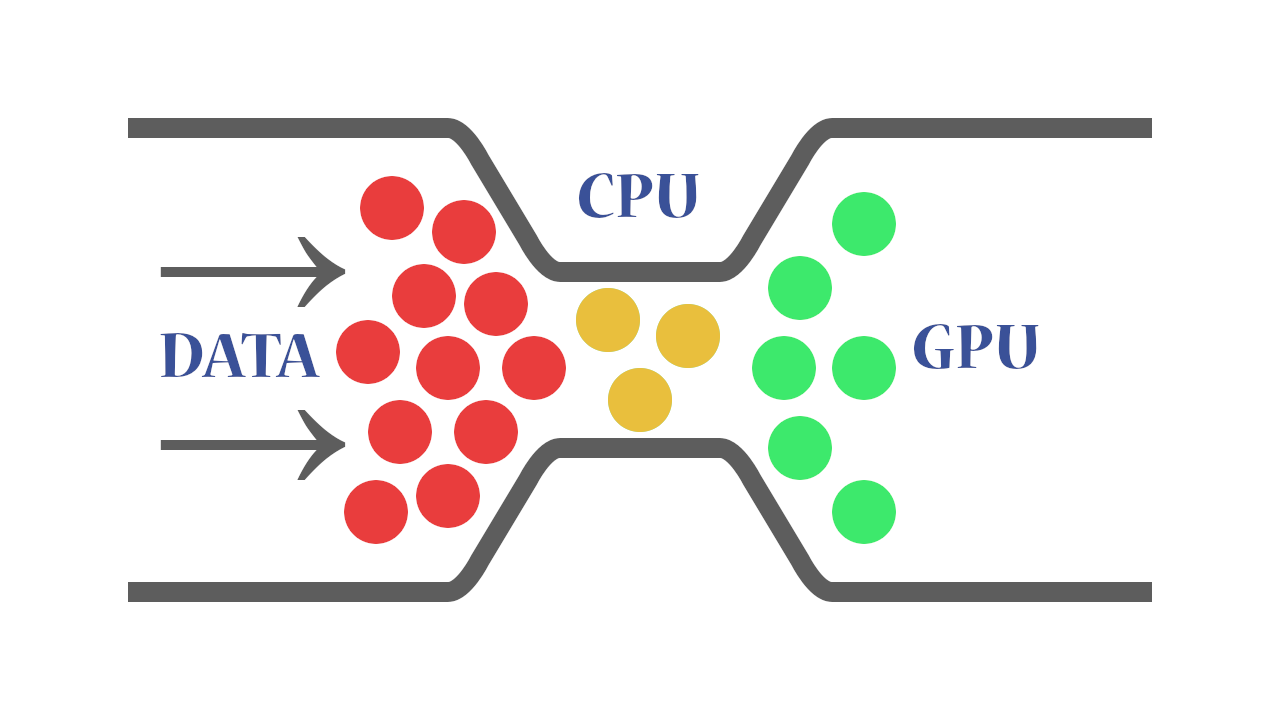
\includegraphics[width=1\linewidth]{images-pipeline/bottleneck.png}
                    \label{ris:netron}
                    \caption{Иллюстрация потери данных при конвертации CPU->GPU}
                \end{minipage}
            \end{center}
        \end{figure}
        \item Выбрана модель для построения конвейера. Ею стала ESPCN из-за довольно простой архитектуры (три слоя Conv2D, слой Subpixel и слой activation), что дает довольной большой выигрыш при инференсе, так как потери при конвертации данных с CPU на GPU не перекрывают скорость самой обработки. Данная модель реализует эффективный super-resolution в реальном времени;
        \item Сконструирована общая архитектура пайплайна. Она состоит из 4 основных этапов: преобразование модели в удобный для работы формат, загрузка модели и манипуляции с ней, генерация вычислительного графа и необходимая предобработка, выполнение соответствующих операторов для обработки модели;
        \item Согласно разработанной архитектуре, был реализован пайплайн на языке программирования С++, в основе которого лежит движок OpenGL. Также были задействованы следующие сторонние библиотеки: glm (для работы с математическими функциями, необходимыми для OpenGL), OpenCV (для захвата и хранения изображения на CPU стороне), Glad и GLFW (для создания контекста OpenGL и работы с его зависимостями), nlohmann::json (для работы с файлами json);
        \item Написан скрипт для конвертации модели из формата .h5 (формат в котором хранится модель, обученная фреймворком TensorFlow) в json файл. Для более удобного использования данный скрипт написан на языке программирования Python;
        \item Разработана архитектура обработки данных на шейдерах (структура вершинного и пиксельного шейдера). Также написаны шаблоны пиксельных шейдеров для слоев Conv2D, Activation и Subpixel;
        \item Протестирована работоспособность построенного пайплайна.
    \end{enumerate}

    \chapter*{Список использованных источников}
    \addcontentsline{toc}{chapter}{Список использованных источников}
    \begin{enumerate}
        \item \hypertarget{[1]}{}Google AI Edge. (2025). Introducing LiteRT: Google's high-performance runtime for on-device AI, formerly known as TensorFlow Lite [Электронный ресурс]. Google AI Edge. – Режим доступа: \href{https://ai.google.dev/edge/litert}{https://ai.google.dev/edge/litert}. – Дата доступа: 18.04.2025.
        
        \item \hypertarget{[2]}{}PyTorch Foundation. (2025). PyTorch Mobile: End-to-end workflow from Training to Deployment for iOS and Android mobile devices [Электронный ресурс]. PyTorch. – Режим доступа: \href{https://pytorch.org/mobile/home/}{https://pytorch.org/mobile/home/}. – Дата доступа: 18.04.2025.
        
        \item \hypertarget{[3]}{}Apple Inc. (н.д.). Core ML | Apple Developer Documentation [Электронный ресурс]. Apple Inc. – Н/Д: Apple Inc. – Режим доступа: \href{https://developer.apple.com/documentation/coreml/}{https://developer.apple.com/documentation/coreml/}. – Дата доступа: 18.04.2025.
        
        \item \hypertarget{[4]}{}Xiaotang Jiang, Huan Wang, Yiliu Chen, Ziqi Wu, Lichuan Wang, Bin Zou, Yafeng Yang, Zongyang Cui, Yu Cai, Tianhang Yu, Chengfei Lv, Zhihua Wu. (2020). MNN: A Universal and Efficient Inference Engine [Электронный ресурс]: Proceedings of the 3rd MLSys Conference. – Austin, TX, USA, 2020. – Режим доступа: \href{https://arxiv.org/pdf/2002.12418}{https://arxiv.org/pdf/2002.12418}. – Дата доступа: 18.04.2025.

        \item \hypertarget{[5]}{}NCNN Foundation. – Austin, TX, USA, 2020. – Режим доступа: \href{https://github.com/Tencent/ncnn}{https://github.com/Tencent/ncnn}. – Дата доступа: 18.04.2025.

        \item \hypertarget{[6]}{} TNN Foundation. – Режим доступа: \href{https://github.com/Tencent/TNN}{https://github.com/Tencent/TNN}. – Дата доступа: 18.04.2025.

        \item \hypertarget{[7]}{} Bolt AI. Huawei Noah. – Режим доступа: \href{https://zhuanlan.zhihu.com/p/317111024}{https://zhuanlan.zhihu.com/p/317111024}. – Дата доступа: 18.04.2025.

        \item \hypertarget{[8]}{} Mace AI. Xiami. – Режим доступа: \href{https://github.com/XiaoMi/mace}{https://github.com/XiaoMi/mace}. – Дата доступа: 18.04.2025.

        \item \hypertarget{[9]}{} Anakin AI. PaddlePaddle. – Режим доступа: \href{https://github.com/PaddlePaddle/Anakin}{https://github.com/PaddlePaddle/Anakin}. – Дата доступа: 18.04.2025.

        \item \hypertarget{[10]}{} Mace AI. Xiami. – Режим доступа: \href{https://github.com/XiaoMi/mace}{https://github.com/XiaoMi/mace}. – Дата доступа: 18.04.2025.
        
        \item \hypertarget{[11]}{}Shi, W., Caballero, J., Huszar, F., Totz, J., Aitken, A. P., Bishop, R., Rueckert, D., Wang, Z. (2016). Real-Time Single Image and Video Super-Resolution Using an Efficient Sub-Pixel Convolutional Neural Network. [Электронный ресурс]: Twitter, Inc. – Режим доступа: \href{https://arxiv.org/pdf/1707.02937}{https://arxiv.org/pdf/1707.02937}. – Дата доступа: 18.04.2025.

        \item \hypertarget{[12]}{} Netron App. – Режим доступа: \href{https://netron.app}{https://netron.app}. – Дата доступа: 18.04.2025.
        
        \item \hypertarget{[13]}{} Image 1.1. – Режим доступа: \href{https://ars.els-cdn.com/content/image/1-s2.0-S0925231224013997-gr3.jpg}{https://ars.els-cdn.com/content/image/1-s2.0-S0925231224013997-gr3.jpg}. – Дата доступа: 18.04.2025.
        
        \item \hypertarget{[14]}{} Image 2.3. – Режим доступа: \href{https://www.google.com/url?sa=i&url=https%3A%2F%2Ffocuskr.tistory.com%2F446&psig=AOvVaw18hUxOSyXB0tNT-SiyNw04&ust=1745263109378000&source=images&cd=vfe&opi=89978449&ved=0CBQQjRxqFwoTCJDN7-6p54wDFQAAAAAdAAAAABAI}{https://www.google.com/url?sa}. – Дата доступа: 18.04.2025.

        \vspace*{\fill}
        \noindent Студент $\underset{\text{подпись, ФИО}}{\underline{\hspace{13.8cm}}}$
        \noindent \\ Непосредственный руководитель\\ практики от организации $\underset{\text{должность, подпись, ФИО}}{\underline{\hspace{10cm}}}$
        \noindent Руководитель (заместитель руководителя)\\организации $\underset{\text{должность, подпись, ФИО}}{\underline{\hspace{12.8cm}}}$
    \end{enumerate}
    
\end{document}
